\documentclass{standalone}
\usepackage[T1]{fontenc}
\renewcommand*\familydefault{\sfdefault} %%
\usepackage{sfmath}
\usepackage{pgfplots}

\begin{document}
\tikzset{every picture/.style={line width=0.75pt}} %set default line width to 0.75pt        

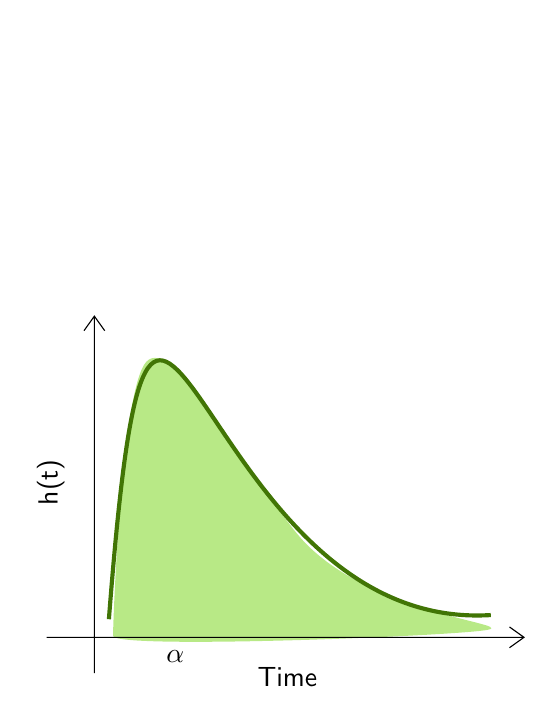
\begin{tikzpicture}[x=0.75pt,y=0.75pt,yscale=-1,xscale=1]
%uncomment if require: \path (0,219); %set diagram left start at 0, and has height of 219

%Shape: Polygon Curved [id:ds5682809837110752] 
\draw  [draw opacity=0][fill={rgb, 255:red, 184; green, 233; blue, 134 }  ,fill opacity=1 ] (52,48) .. controls (64,35) and (93,91) .. (124,130) .. controls (155,169) and (229,174) .. (217,177) .. controls (205,180) and (36,186.73) .. (36,180) .. controls (36,173.27) and (40,61) .. (52,48) -- cycle ;
%Shape: Axis 2D [id:dp7984867080871099] 
\draw  (4,180.73) -- (234,180.73)(27,26) -- (27,197.92) (227,175.73) -- (234,180.73) -- (227,185.73) (22,33) -- (27,26) -- (32,33)  ;
%Curve Lines [id:da9511293985094285] 
\draw [color={rgb, 255:red, 65; green, 117; blue, 5 }  ,draw opacity=1 ][line width=1.5]    (34,172) .. controls (56,-112) and (72,179) .. (218,170) ;
% Text Node
\draw (6,106) node [rotate=-270.08] [align=left] {h(t)};
% Text Node
\draw (66,190) node  [align=left] {$\alpha$};
\draw (120,200) node  [align=left] {Time};

\end{tikzpicture}

\end{document}